\chapter{Introdução}

Os fenômenos de transferência são um campo de estudo que se baseia em compreender como ocorre o transporte de calor, momento, massa, entre outras grandezas físicas, num dado fluido ou meio em análise \citep{1,2,3}. No tocante à transferência de massa, a difusão é um dos mecanismos mais comuns, cuja força motriz está condicionada à presença de um gradiente de concentração em relação à uma ou mais espécies químicas no volume de controle estudado \citep{2,3}. A difusão está presente nos mais variados contextos: processos químicos industriais com reação química, processos físicos de separação, transporte de oxigênio, nutrientes e íons por membranas celulares, no mecanismo de ação de fármacos, entre outros \citep{2}.

Este fenômeno de transferência de matéria pode ocorrer pela movimentação de átomos, íons, moléculas ou até mesmo macromoléculas e sempre se dá contra o gradiente de concentração, isto é, ocorre do ponto de maior concentração química para o de menor. Embora a difusão seja mais lenta e dificultada nos sólidos, em líquidos, gases e vapores ela pode ser mais facilmente observada e medida experimentalmente \citep{2,3,4}.

Um dos pioneiros no estudo da difusão foi o físico alemão Adolf Fick, quem no século XIX postulou duas leis que modelam em linguagem matemática este fenômeno físico. A primeira lei de Fick se baseia na premissa que a relação entre o gradiente de concentração da espécie química e a taxa de transferência de massa observada no sistema é linear. Além disso, analogamente a outros fenômenos de transporte, a difusão pressupõe uma constante de proporcionalidade, que é intrínseca a uma determinada espécie em um meio específico. Esta constante é conhecida como coeficiente de difusão ou difusividade e seu significado físico é mensurar a capacidade de mobilidade que uma determinada espécie de soluto tem num solvente em particular \citep{2,4}. Esta lei pode ser representada como: 


\begin{equation}\label{key}
J_{A}=-C D_{A B} \nabla y_{A}
\end{equation}

onde:

\begin{itemize}
	\item $J_{A}$ é o fluxo difusivo molar de uma espécie química A $[\frac{kmol}{sm^{2}}]$;
	\item C é a concentração molar total da mistura [$\frac{kmol}{m^{3}}]$;
	\item $D_{AB}$ é a difusividade mássica $[\frac{m^{2}}{s}]$;
	\item $\nabla y_{A}$ é o gradiente de fração molar da espécie química A $[\frac{1}{m}]$.
\end{itemize}

Além disso, em muitos casos, quando a concentração da espécie varia com o tempo, não se verifica mais uma relação linear tal como na primeira Lei de Fick, neste caso é mais adequada a segunda Lei de Fick, que leva em conta esta premissa.

Neste estudo, um aparato experimental foi usado para estimar o coeficiente de difusão do diclorometano em ar, compostos doravante denominados A e B, respectivamente. Determinou-se a concentração de A em dois pontos, usando-se um ventilador para garantir a dispersão de A em B, isto é, obter concentração de A nula. Ademais, assumiu-se que a difusão é unidimensional (vertical), unimolecular (B não difunde em A), estado pseudo estacionário e que $D_{AB}$ não varia ao longo do processo.
\\

\chapter{Objetivos}

Medir experimentalmente a difusividade mássica $D_{AB}$ do diclorometano (A) em ar (B) a $28^{o} C$ e 1 atm, e comparar o valor estimado com valores tabelados e correlações da literatura.
\\

\chapter{Materiais e Equipamentos}

\section{Materiais}

Os materiais utilizados para a realização do experimento foram:

\begin{itemize}
\item	Célula Arnold
\item	Ventilador
\item	Termômetro
\item	Papel milimetrado
\item	Banho Termostático
\item	Suporte
\item	Cronômetro
\item	Diclorometano
\end{itemize}

\section{Equipamento}

\begin{figure}[H]
	\begin{center}
		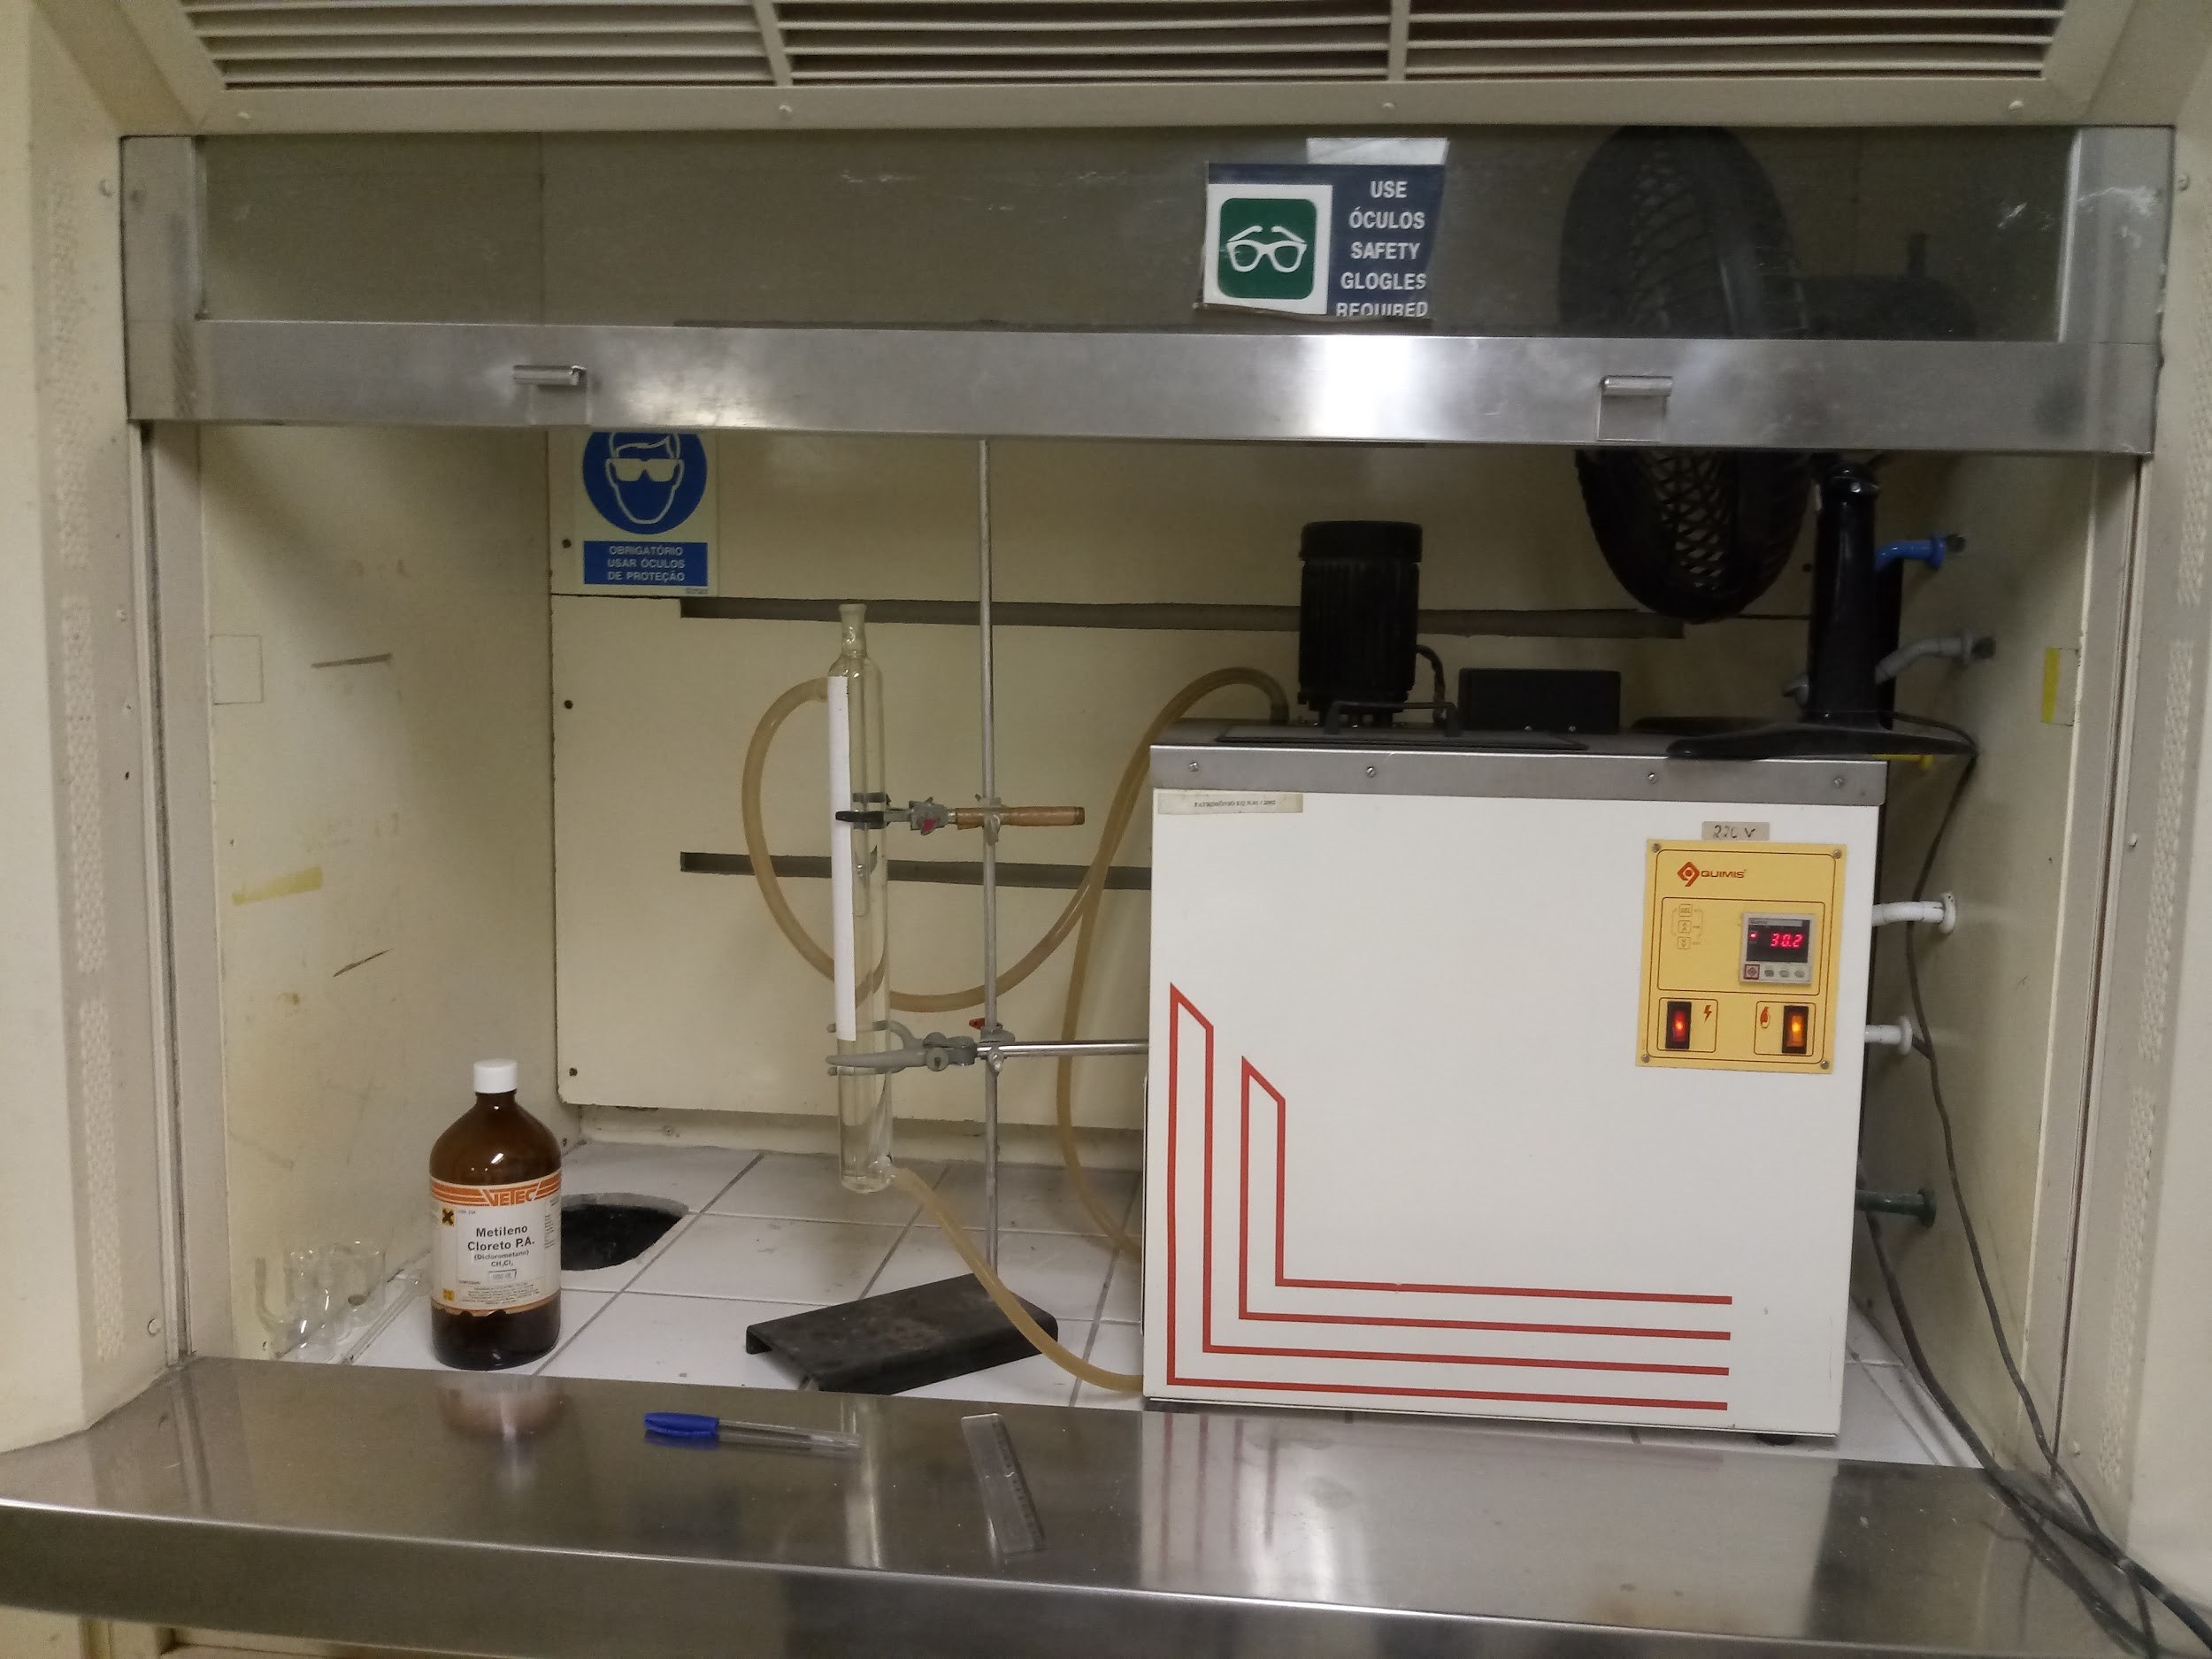
\includegraphics[scale=0.2,trim={0 0 0 0}]{figuras/ladeq/difusao/aparato}
		%\vspace{-20pt}
		\caption{Equipamento utilizado para o experimento}
		\label{apa}
	\end{center}
\end{figure}


\chapter{Procedimento}

O sistema conhecido como célula de Arnold foi utilizado para a realização do experimento. Ela é constituída por um tubo interno, no qual coloca-se o líquido cuja difusividade se deseja determinar e por um tubo externo onde a água do banho termostatizado circula para manter a temperatura do sistema em torno de $28^{o}$ C.

O diclorometano foi colocado no recipiente e o menisco formado foi considerado o zero da escala. A cada intervalo de 15 minutos foram tomadas as medidas de temperatura e variação de massa do diclorometano. Após o período de 1 hora, deu-se por encerrado o experimento.
\\

\chapter{Descrição teórica do sistema}

A Célula de Arnold, esquematizada na Figura \ref{apaTeo}, pode ser usada para determinar o coeficiente de difusão de uma determinada amostra. Para a realização do experimento, a temperatura e a pressão são mantidas constantes. Em um tubo estreito com indicação de nível, parcialmente cheio com um líquido A (neste caso, diclorometano), vaporiza e se difunde na fase gasosa (ar). A razão de vaporização pode ser fisicamente determinada e matematicamente expressa em termos de fluxo molar. O gás, além de possuir uma insignificante solubilidade no líquido A, também é quimicamente inerte ao mesmo.
Tendo em vista que a concentração molar do líquido é muito maior do que a concentração da fase gasosa, considera-se a velocidade da interface gás-líquido desprezível. A presente condição é chamada de estado quase estacionário. Desta forma, o balanço de massa desse sistema de controle para um estado estacionário é:

\begin{equation}\label{key}
A \times N_{A, Z|Z+\Delta Z}-A \times N_{A, Z | Z}=0
\end{equation}

\begin{figure}[H]
	\begin{center}
		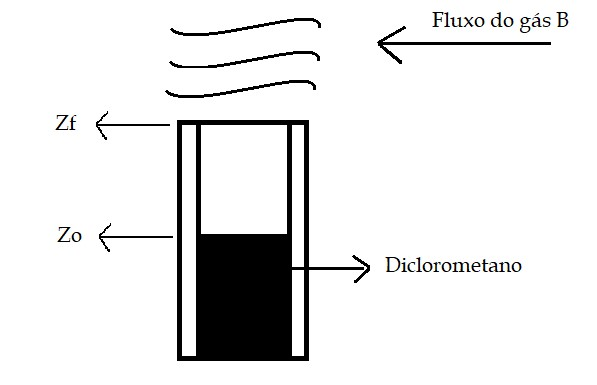
\includegraphics[scale=0.6,trim={0 0 0 0}]{figuras/ladeq/difusao/aparatoTeo}
		%\vspace{-20pt}
		\caption{Esquema da Célula de Arnold}
		\label{apaTeo}
	\end{center}
\end{figure}



\section{Considerações do modelo}



\begin{itemize}

\item Mistura binária;
\item Temperatura e pressão constantes;
\item Estado Pseudo-estacionário $\frac{DC_A}{dt}= 0$;
\item $D_{AB}$ não varia ao longo do processo difusivo;
\item Modelo de Fick é válido;
\item Difusão unidimensional (apenas o diclorometano se difunde);
\item Sistema homogêneo;
\item Não há reação química $r_A=0$;
\item O ar é insolúvel no diclorometano.

\end{itemize}

Desta forma, pelo modelo de Fick e aplicando a conservação de massa na fase gasosa, temos que:

Sabe-se que as moléculas se movem de forma aleatória ao longo do espaço disponível. Entretanto na aleatoriedade do movimento é possível observar um comportamento de conjunto que favorece um fluxo de partículas no sentido que sai da região de maior concentração para aa região com menor concentração. Dessa interpretação, surge o conceito básico de \emph{fluxo molar difusivo}, dado pela primeira lei de Fick: 

\begin{equation}\label{key}
J_{A}=-D_{A B} \nabla C_{A}
\end{equation}

Como no presente experimento, considera-se que a difusão ocorre apenas no sentido vertical, com orientação para cima, a lei assume a forma:

\newpage

%\begin{equation}\label{key}
%\mathrm{J}_{\mathrm{A}}=-\mathrm{D}_{\mathrm{AB}} \partial \mathrm{C}_{\mathrm{A}} \partial z
%\end{equation}

\begin{equation}\label{key}
\mathrm{J}_{\mathrm{A}}=-\mathrm{D}_{\mathrm{AB} } \dfrac{\partial \mathrm{C}_{\mathrm{A}}}{\partial z} 
\end{equation}


$D_{AB}$ - é a constante de proporcionalidade chamada coeficiente de difusão

Esse transporte de matéria causado pelo movimento das partículas pode também ser representado considerando a concentração das mesmas associadas à sua velocidade média, que pode ser escrita da forma: 


\begin{equation}\label{key}
\mathrm{J}_{\mathrm{A}}=\mathrm{C}_{\mathrm{A}}\left(\mathrm{v}_{\mathrm{A}, \mathrm{z}}-\mathrm{V}_{\mathrm{z}}\right)
\end{equation}


onde: 

\begin{itemize}
	\item $\mathrm{v}_{\mathrm{A}, \mathrm{z}}$: velocidade média de A na direção z.
	\item $V_{z}$: velocidade média da solução como um todo, também em z, dada para dois componentes por: 
	\begin{itemize}
		\item $V_{z}=\frac{1}{C}\left(C_{A} V_{A, z}-V_{z}\right)+C_{A} V_{z}=C_{A} V_{A, x}$
	\end{itemize}
\end{itemize}


O fluxo molar difusivo associado ao convectivo geram o fluxo molar total que é representado por:

\begin{equation}\label{key}
N_{A}=-C D_{A B} \frac{\partial Y _{A}}{\partial z}+Y_{A}\left(N_{A}+N_{B}\right)
\end{equation}

Tendo em vista que $N_{B} = 0$:

\begin{equation}\label{key}
N_{A}=-C D_{A B} \frac{\partial Y _{A}}{\partial z}+Y_{A} N_{A}
\end{equation}
\newpage

Que reescrita fica:

\begin{equation}\label{key}
N_{A}=\frac{C D _{A B}}{Z_{2}-Z_{1}} \ln \left(\frac{1-Y _{A 2}}{1-Y _{A 1}}\right), Z_{2}=Y_{A 2}=0
\end{equation}

Pela equação de balanço na interface:

\begin{equation}\label{key}
\frac{2 C _{A}}{\partial t}+\frac{2 N _{A}}{\partial z}=0 \operatorname{com} N_{A}=-C D_{A B} \frac{1}{1-Y _{A}} \frac{d Y _{A}}{d z}
\end{equation}

Realizando o balanço de massa na interface,

\begin{equation}\label{key}
\mathrm{N}_{\mathrm{A}}=\mathrm{C}_{\mathrm{A}}\left.\mathrm{v}_{\mathrm{A}}\right|_{z} \mapsto \mathrm{C}_{\mathrm{AL}} \frac{d L}{d t}
\end{equation}

Por fim, temos:

\begin{equation}\label{key}
N_{A}=C_{A L} \frac{d L}{d t}=\frac{C D_{AB}}{L} \ln \left(\frac{1}{Y _{A 1}}\right)=-C D_{A B} \ln \left(1-Y_{A 1}\right)
\end{equation}

Realizando a integral, encontra-se

\begin{equation}\label{key}
L^{2}-L_{0}^{2}=-2 \frac{\frac{C D _{A B}}{C_{A L}}} \ln \left(1-Y_{A 1}\right) t
\end{equation}

Por meio da obtenção do comportamento da altura ao longo do tempo, é possível realizar o cálculo de DAB. 
\\

\chapter{Determinação do Coeficiente de Difusão}


\section{Cálculo Teórico}

Foram usadas duas equações para o cálculo teórico do coeficiente de difusão.
A primeira foi a equação semi-empírica proposta por \citep{Fuller}. Foi reportado em literatura que a predição apresenta erros em torno de 7\% e pode ser usada tanto para pares de gases polares como apolares.


\begin{equation}\label{key}
D_{A B}=\frac{1.0 \times 10^{-9} T^{1.75}}{P\left[\left(\sum v\right)_{A}^{1 / 3}+\left(\sum v\right)_{B}^{1 / 3}\right]^{2}}\left(\frac{1}{M_{A}}+\frac{1}{M_{B}}\right)^{1 / 2}
\end{equation}


onde:

\begin{itemize}

\item T é a temperatura em K

\item P é a pressão em atm

\item $M_{A}$ e $M_{B}$ é a massa molar das substâncias,

\item $\Sigma_{v}$ é a soma dos volumes atômicos dos elementos de cada molécula (obtidos da tabela 2-2 do Hines e Maddox)

\end{itemize}

O valor calculado por Fuller foi de $1,07 \times 10^{-5} [\dfrac{m^{2}}{s}]$.

Uma segunda equação foi a de Chapman-Enskog, que é recomendada para pares de gases apolares. 

\begin{equation}\label{key}
D_{A B}=\frac{1.858 \times 10^{-27} T^{3 / 2}}{P \sigma_{A B}^{2} \Omega_{D}}\left(\frac{1}{M_{A}}+\frac{1}{M_{B}}\right)^{1 / 2}
\end{equation}

onde:

\begin{itemize}

\item $D_{AB}$ é a difusividade, $\dfrac{m^{2}}{s}$;
\item T é a temperatura absoluta, K;
\item M é a massa molecular, $\dfrac{kg}{kgmol}$;
\item P é a pressão absoluta, atm;
\item $\sigma_{AB}$ é o diâmetro de colisão, m;
\item $\Omega_{D}$ integral de colisão.

\end{itemize}



\begin{equation}\label{key}
\Omega_{D}=\left(44.54 T^{\sigma-4.909}+1.911 T^{\sigma-1.575}\right)^{0.10}
\end{equation}

Brokaw propôs uma correção no valor da integral de colisão ($\Omega_{D}$) considerando o momento de dipolo das moléculas, para calcular o coeficiente de difusão para pares de moléculas polares. No entanto, como neste caso temos uma molécula polar (diclorometano) e uma mistura apolar (ar) o fator $\delta_{A B}$ é 0, o que faz com que a integral de colisão para esse caso seja calculada da maneira prevista por Chapman e Enskog.

Correções de Brokaw:

\begin{itemize}
\item $\Omega_{D^{\sigma}}=\Omega_{D}+0.19 \delta_{A \beta}^{2} / T^{\circ}$

\item $\sigma_{A B^{\sigma}}=\left(\sigma_{A} \cdot \sigma_{B^{*}}\right)^{1 / 2}$

\item $\delta_{A B}=\left(\delta_{A} \delta_{B}\right)^{1 / 2}$

\item $\varepsilon_{A B^{\sigma}}=\left(\varepsilon_{A^{\sigma}} \varepsilon_{B^{\sigma}}\right)^{1 / 2}$

\item $\delta=\frac{1.94 \times 10^{3} \mu_{p}^{2}}{V_{b} T_{b}}$

\end{itemize}


\begin{figure}[H]
	\begin{center}
		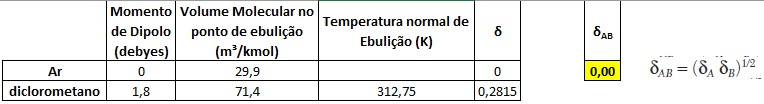
\includegraphics[scale=0.8,trim={0 0 0 0}]{figuras/ladeq/difusao/tab1}
		%\vspace{-20pt}
		\caption{Dados usados para o cálculo.}
		\label{tab1}
	\end{center}
\end{figure}


\begin{figure}[H]
	\begin{center}
		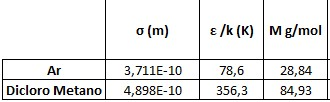
\includegraphics[scale=0.8,trim={0 0 0 0}]{figuras/ladeq/difusao/tab2}
		%\vspace{-20pt}
		\caption{Dados usados para o cálculo.}
		\label{tab2}
	\end{center}
\end{figure}


Dadas as considerações, o coeficiente de difusão calculado pela equação de Chapman-Enskog foi de $1,023 \times 10^{-5}  \dfrac{m^{2}}{s}$.

\chapter{Resultados e Discussão}

\section{Dados Experimentais}

Foi observado durante o experimento que a temperatura do banho não se manteve constante no valor ajustado no controlador de temperatura do equipamento. A temperatura foi ajustada para o valor de $28^{\circ} C$. A variação da temperatura marcada pelo controlador pode ser observada no gráfico da Figura \ref{temp}.


\begin{figure}[H]
	\begin{center}
		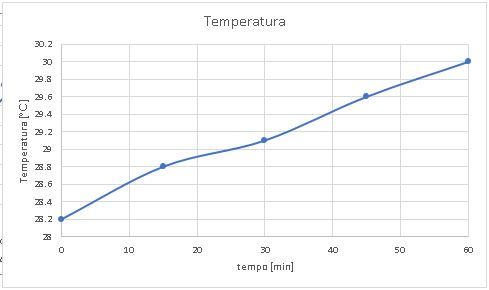
\includegraphics[scale=0.8,trim={0 0 0 0}]{figuras/ladeq/difusao/tempGraph}
		%\vspace{-20pt}
		\caption{Variação da temperatura ao longo do experimento.}
		\label{temp}
	\end{center}
\end{figure}

A principal variável de modelagem do experimento é a altura ou nível de diclorometano dentro da célula de Arnold. A dados coletados no experimento podem ser observados no gráfico da Figura \ref{diclo}.




\begin{figure}[H]
	\begin{center}
		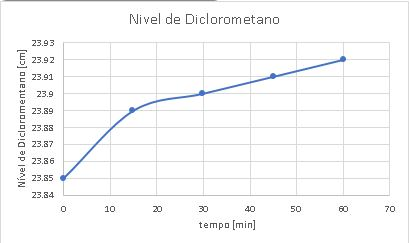
\includegraphics[scale=1,trim={0 0 0 0}]{figuras/ladeq/difusao/nivelDiclo}
		%\vspace{-20pt}
		\caption{Variação do nível de diclorometano com altura corrigida.}
		\label{diclo}
	\end{center}
\end{figure}

Para melhor visualização da variação do nível, calculou-se a variação do nível de diclorometano em relação ao nível inicial na célula de Arnold. Conforme podemos ver no gráfico da Figura \ref{delta} a variação total no nível foi menor do que o esperado e isso pode ter fonte de erros para os valores calculados. A pequena variação pode ser atribuída à algumas causas, como:

\begin{itemize}
	\item Quantidade de diclorometano inicial muito pequena;
	\item Contaminação do diclorometano.
\end{itemize}

Estas hipótese foram levantadas, pois a montagem do aparato e a preparação da carga de diclorometano foi realizada muito antes do início do experimento. Isso gerou algumas incertezas quanto a composição do líquido presente na célula de Arnold. A falta de diclorometano no estoque também impossibilitou o experimento com um nível inicial maior.

\begin{figure}[H]
	\begin{center}
		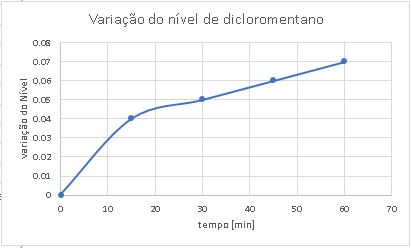
\includegraphics[scale=1,trim={0 0 0 0}]{figuras/ladeq/difusao/delta}
		%\vspace{-20pt}
		\caption{Variação do nível de diclorometano com altura corrigida.}
		\label{delta}
	\end{center}
\end{figure}


A partir dos dados experimentais foram então calculados os coeficientes de difusão para comparação com os dados encontrados na literatura.

\section{Determinação do coeficiente de difusão experimental}

Primeiramente é necessário calcular a pressão de saturação do diclorometano nas condições do experimento. Considerando a temperatura de $28 ^{\circ}$ C e pressão atmosférica de 1 atm.

Dados:

\begin{itemize}
	\item Temperatura: 303,15 [K];
	\item Pressão: $1,01325 \times 10^{5} [\mathrm{Pa}]$
\end{itemize}

\begin{equation}\label{key}
\ln P s a t=A-\frac{B}{T+C}
\end{equation}

O parâmetros utilizados e o valor calculado para a pressão de saturação pode ser observado na Tabela \ref{tab:sat}

\begin{table}[H]
	\centering
	\begin{tabular}{|l|l|l|}
		\hline
		\multicolumn{3}{|c|}{\textbf{Cálculo de Psat}} \\ \hline
		\textbf{T} & 28 & °C \\ \hline
		\textbf{A} & 13.9891 &  \\ \hline
		\textbf{B} & 2463.93 &  \\ \hline
		\textbf{C} & 223.24 &  \\ \hline
		\textbf{ln Psat} & 4.18 &  \\ \hline
		\textbf{Psat} & 65.50 & kPa \\ \hline
	\end{tabular}
	\caption{Cálculo da pressão de Saturação}
	\label{tab:sat}
\end{table}

A partir da pressão de saturação foram calculados os valores de concentração de diclorometano próxima a interface líquido-ar. Foram utilizadas as seguintes fórmulas:

\begin{equation}\label{key}
y_{A i}=\frac{P_{A}^{SAT}(T)}{P}
\end{equation}

\begin{equation}\label{key}
C=\frac{P}{R T}
\end{equation}

A concentração de diclorometano na fase líquida poder ser calculada por:

\begin{equation}\label{key}
C_{A, L}=\frac{\rho_{A, L}}{M_{A}}
\end{equation}

E finalmente o cálculo do coeficiente de difusão é obtido através da equação:


\begin{equation}\label{key}
D_{A B}=\frac{\text {coef.angular} \cdot C_{A L}}{-2 \cdot C \cdot \ln \left(1-y_{A i}\right)}
\end{equation}

O coeficiente angular é dado pela seguinte equação:

\begin{equation}\label{key}
\text {coef.angular}=\frac{L^{2}-L_{0}^{2}}{t}
\end{equation}

Ou seja, o coeficiente angular foi obtido através da regressão dos dados experimentais.


\section{Ajuste linear para altura corrigida}


Na Figura \ref{linear} podemos observar a reta obtida através dos dados de altura no nível de diclorometano corrigida com a altura do bocal da célula de Arnold.

\begin{figure}[H]
	\begin{center}
		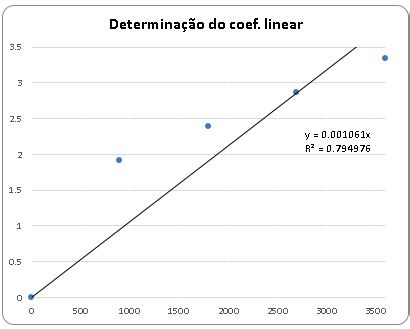
\includegraphics[scale=1,trim={0 0 0 0}]{figuras/ladeq/difusao/linear00}
		%\vspace{-20pt}
		\caption{Regressão dos dados experimentais para obtenção do coeficiente angular.}
		\label{linear}
	\end{center}
\end{figure}

A Tabela \ref{tab:dif} apresenta os cálculos para a obtenção do coeficiente de difusão experimental.


\begin{table}[H]
		\centering
	\begin{tabular}{|l|l|l|}
		\hline
		\multicolumn{3}{|c|}{\textbf{Cálculos}} \\ \hline
		Psat & 65498.23 & Pa \\ \hline
		$y_{A1}$ & 0.6464 &  \\ \hline
		C & 40.47 & mol/m³ \\ \hline
		$C _{AL}$ & 15659.96 & mol/m³ \\ \hline
		\begin{tabular}[c]{@{}l@{}}Coeficiente exp\end{tabular} & 1.06E-03 &  \\ \hline
		\multicolumn{1}{|c|}{\multirow{2}{*}{$D_{AB}$}} & 1.98E-01 & cm²/s \\ \cline{2-3} 
		\multicolumn{1}{|c|}{} & 1.98E-05 & m²/s \\ \hline
	\end{tabular}
	\caption{Cálculo do coeficiente de difusão.}
	\label{tab:dif}
\end{table}

\section{Ajuste linear para altura medida}

Na Figura \ref{linear2} podemos observar a reta obtida através dos dados de altura no nível de diclorometano sem a correção com a altura do bocal da célula de Arnold.

\begin{figure}[H]
	\begin{center}
		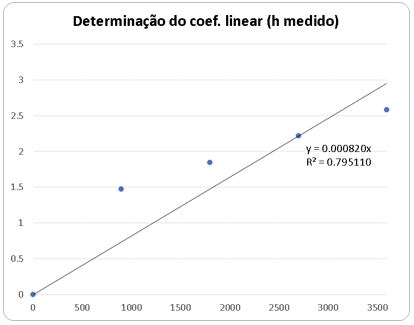
\includegraphics[scale=1,trim={0 0 0 0}]{figuras/ladeq/difusao/linear002}
		%\vspace{-20pt}
		\caption{Regressão dos dados experimentais para obtenção do coeficiente angular.}
		\label{linear2}
	\end{center}
\end{figure}

A Tabela \ref{tab:dif2} apresenta os cálculos para a obtenção do coeficiente de difusão experimental.


\begin{table}[H]
	\centering
	\begin{tabular}{|l|l|l|}
		\hline
		\multicolumn{3}{|c|}{\textbf{Cálculos}} \\ \hline
		Psat & 65498.23 & Pa \\ \hline
		$y_{A1}$ & 0.6464 &  \\ \hline
		C & 40.47 & mol/m³ \\ \hline
		$C _{AL}$ & 15659.96 & mol/m³ \\ \hline
		\begin{tabular}[c]{@{}l@{}}Coeficiente exp\end{tabular} & 8.20E-04 &  \\ \hline
		\multicolumn{1}{|c|}{\multirow{2}{*}{$D_{AB}$}} & 1.53E-01 & $cm^{2}/s$ \\ \cline{2-3} 
		\multicolumn{1}{|c|}{} & 1.53E-05 & $m^{2}/s$ \\ \hline
	\end{tabular}
	\caption{Cálculo do coeficiente de difusão.}
	\label{tab:dif2}
\end{table}


\chapter{Análise dos Resultados}


Comparando-se os valores de $D_{AB}$ obtidos experimentalmente, percebemos que quando desconsideramos a altura entre o papel milimetrado e a abertura do tubo, o valor do coeficiente de difusão obtido é menor do que quando considerado $(1,98 \times 10^{-5} m^{2}/s$ e $1,53 \times 10^{-5} m^{2}/s$, respectivamente), o que pode ser explicado pelo fato de estarmos subestimando o caminho difusivo percorrido pelo gás, então o valor do coeficiente de difusão deve ser menor. Já ao comparar os valores de $D_{AB}$ obtidos experimentalmente com os valores teóricos, o valor calculado (considerando a altura) foi maior do que os valores teóricos (\citep{Fuller}: $ 07 \times 10^{-5} m^{2}/s; Chapman-Enskog: 1,023 \times 10^{-5} m^{2}/s$), algo inesperado pelo menos de acordo com o objetivo da prática, em que os valores deveriam ser próximos dos valores teóricos, com porcentagem de erro considerável. Mesmo assim, o resultado e as condições da prática confirmam o valor diferente dos valores teóricos, cuja informação pôde ser concretizada com o valor do $R^{2}$ gerado no gráfico do cálculo do coeficiente de difusão ($R^{2}$ = 0,795110, o qual deveria ser próximo de 1,0).

Diversos motivos podem ter sido responsáveis por essa diferença no valor do coeficiente de difusão, sendo possível citar, por exemplo, erros na leitura das alturas do diclorometano ao longo do tempo, visto que tal leitura foi realizada individualmente por cada componente do grupo, para depois obterem-se os respectivos valores médios, sendo que tais leituras deveriam ter sido tomadas de forma rápida, já que estavam variando constantemente, sem contar que a escala utilizada em papel milimetrado era imprecisa. Além disso, como a temperatura ao longo do experimento não se manteve constante, isso deve ter gerado erros na medição da mesma por parte do aparelho, não esquecendo das hipóteses e aproximações realizadas nos cálculos de $D_{AB}$, que podem gerar outros pequenos erros. Contudo, a hipótese mais plausível e considerável para o experimento foi o fato de que o diclorometano pode ter sido contaminado, o que impossibilitou a credibilidade e, consequentemente, uma análise adequada do experimento, mesmo o valor do coeficiente de difusão experimental obtido estando dentro da faixa de ordem de grandeza esperada para coeficientes de difusão de gases ($10^{-5}$ a $10^{-6} m^{2}/s$).
\\

\chapter{Conclusão}

Através do experimento realizado, foi possível observar o fenômeno de difusão do diclorometano em ar, permitindo obter dados para plotar um gráfico que resultou no cálculo do coeficiente de difusão mássica do conjunto de componentes. O valor encontrado deve ser desconsiderado, mesmo se encontrando dentro da faixa de valores de coeficientes de difusão para gases, visto que houve uma contaminação do diclorometano, impossibilitando a análise e devida comparação do resultado com os modelos teóricos propostos e, por conta disso, o experimento deve ser repetido.
